\documentclass[./main.tex]{subfiles}

\begin{document}
\chapter{ SYSTEM ANALYSIS}
\noindent
System Analysis is the process of studying a procedure or business in order to identify its goals and purposes and create systems and procedures that will achieve them in an efficient way. It is a problem-solving technique that improves the system and ensures that all components of the system work efficiently to accomplish their purpose. 
Analysis specifies what the system should do. This Chapter describes the system analysis of the project. It includes the feasibility study, requirement analysis, and system design.
\addtocontents{lof}{\protect\addvspace{-10pt}}
\addtocontents{lot}{\protect\addvspace{-10pt}}
\section{Requirement Engineering}
Based on our background study and literature review (refer to Chapter \ref{chap:background}), we've identified several projects similar to ours that employ different methodologies and algorithms. Although our project shares similarities with these endeavors, it's essential to clarify that our primary objective does not revolve around the development of a commercial application. Instead, due to time constraints, we will not be incorporating multiple algorithms.

\noindent
As a result of this, we have compiled the following set of requirements for our Stock Price Prediction Application.
\subsection{Functional Requirements}
Functional requirements specify the specific functions, features, and capabilities a system or software must have to meet user needs and perform its intended tasks.

\begin{enumerate}[label=\roman*.]
  \item \textbf{Data Collection and Integration:}
    \begin{itemize}
      \item The system should gather historical stock price data from NEPSE .
    \end{itemize}
  
  \item \textbf{Data Preprossing:}
    \begin{itemize}
      \item The system should clean and preprocess raw data, handling missing values and outliers.
      \item It should normalize or scale data appropriately for modeling.
    \end{itemize}
    
  \item \textbf{Prediction Models:}
    \begin{itemize}
      \item The system should implement LSTM model for prediction .
    \end{itemize}
  
  \item \textbf{Training and Testing:}
    \begin{itemize}
      \item The system should split data into training and testing datasets.
      \item It should provide options for cross-validation and model evaluation.
    \end{itemize}
  \item \textbf{Visualization:}
    \begin{itemize}
      \item The system should offer interactive charts and visualizations of historical and predicted stock prices.
      \item Users should be able to customize the time range and parameters displayed.
    \end{itemize}
\end{enumerate}
\subsection{Non-Functional Requirements : }


\begin{enumerate}[label=\roman*.]
  \item \textbf{Accuracy and Precision:}
    \begin{itemize}
      \item The system should achieve a specified level of accuracy in stock price predictions.
      \item Precision requirements should be defined to minimize false positives in alerting.
    \end{itemize}
    
  \item \textbf{Scalability:}
    \begin{itemize}
      \item The system should handle a growing volume of data and users without performance degradation.
      \item It should support parallel processing or distributed computing for scalability.
    \end{itemize}
    
  \item \textbf{Reliability:}
    \begin{itemize}
      \item The system should be available and reliable 24/7 to support real-time trading decisions.
      \item Redundancy and failover mechanisms should be in place to minimize downtime.
    \end{itemize}
    
  \item \textbf{Response Time:}
    \begin{itemize}
      \item The system should provide real-time or near-real-time predictions and alerts.
      \item Response time requirements should be specified for different functions.
    \end{itemize}
    
  \item \textbf{User Interface:}
    \begin{itemize}
      \item The user interface should be intuitive and user-friendly, catering to both novice and experienced users.
      \item Accessibility and usability guidelines should be followed.
    \end{itemize}
 \end{enumerate}
\section{Feasibility Study} 
 A feasibility study is a comprehensive analysis conducted to assess the practicality and viability of a proposed project, system, product, or business idea. It serves as a critical tool for decision-making, helping stakeholders determine whether a project should be pursued, modified, or abandoned. The primary objectives of a feasibility study are to evaluate the project's potential for success, identify potential challenges, and provide a basis for informed decision-making. 
 
\subsection{Technical Feasibility}
 In the technical aspect of our system, which relies on algorithmic and machine learning models, we will utilize \textbf{Python} as our primary programming language. We'll leverage essential libraries such as \textbf{Pandas, Numpy, Keras, and scikit-learn} to support our core functionalities. As the system grows and evolves, there may be a need to incorporate additional programming languages like JavaScript, and markup languages like HTML and CSS to facilitate further expansion and enhance the user interface.

\subsection{Operational Feasibility}
 For our stock prediction system, operational feasibility means making sure we have the right teammates who understand Python, machine learning, and web technologies. We also need to check that our computers and internet systems can handle the work. We must make sure our data is managed well, and we follow the rules about data privacy. We'll need plans to keep the system running, and handle any future growth. If we can do all this, our stock prediction system will work smoothly and give us the information we need.

\subsection{Economical Feasibility}
The primary expenses associated with developing the system revolve around ensuring that we have adequately equipped devices and a reliable internet connection. Our economic viability also encompasses costs related to travel, wages for staff during system launch, as well as expenses for meals. Additionally, it includes spending on online courses and books for research and study purposes. Deployment costs are another aspect of our economic feasibility plan, along with potential expenses for accessing third-party system APIs.

 % For generating dummy text, remove in your actual document
\begin{center}

\begin{table}[H]
\begin{tabularx}{\textwidth}{|X|X|}
\hline
\textbf{Cost/Revenue Item} & \textbf{Amount (NRs:)} \\
\hline
Initial Investment & 5,000 \\
Internet and Device Costs & 25,000 \\
Travel Expenses & 4,500 \\
Staff Wages (Launch Phase) & 15,000 \\
Research Materials (Courses, Books) & 7,500 \\
Deployment Costs & 3,000 \\
Third-Party API Expenses & 1,200 \\
\hline
\textbf{Total Costs} & 61,200 \\
\hline
Projected Sales/Income & 20,000 \\
\hline
\textbf{Break-Even Point (BEP)} & 41,200 \\
\hline
\end{tabularx}
\caption{Break-Even Analysis}
\end{table}
\end{center}
\newpage
\section{Use Case Diagram}

\begin{figure}[H]
     \centering
     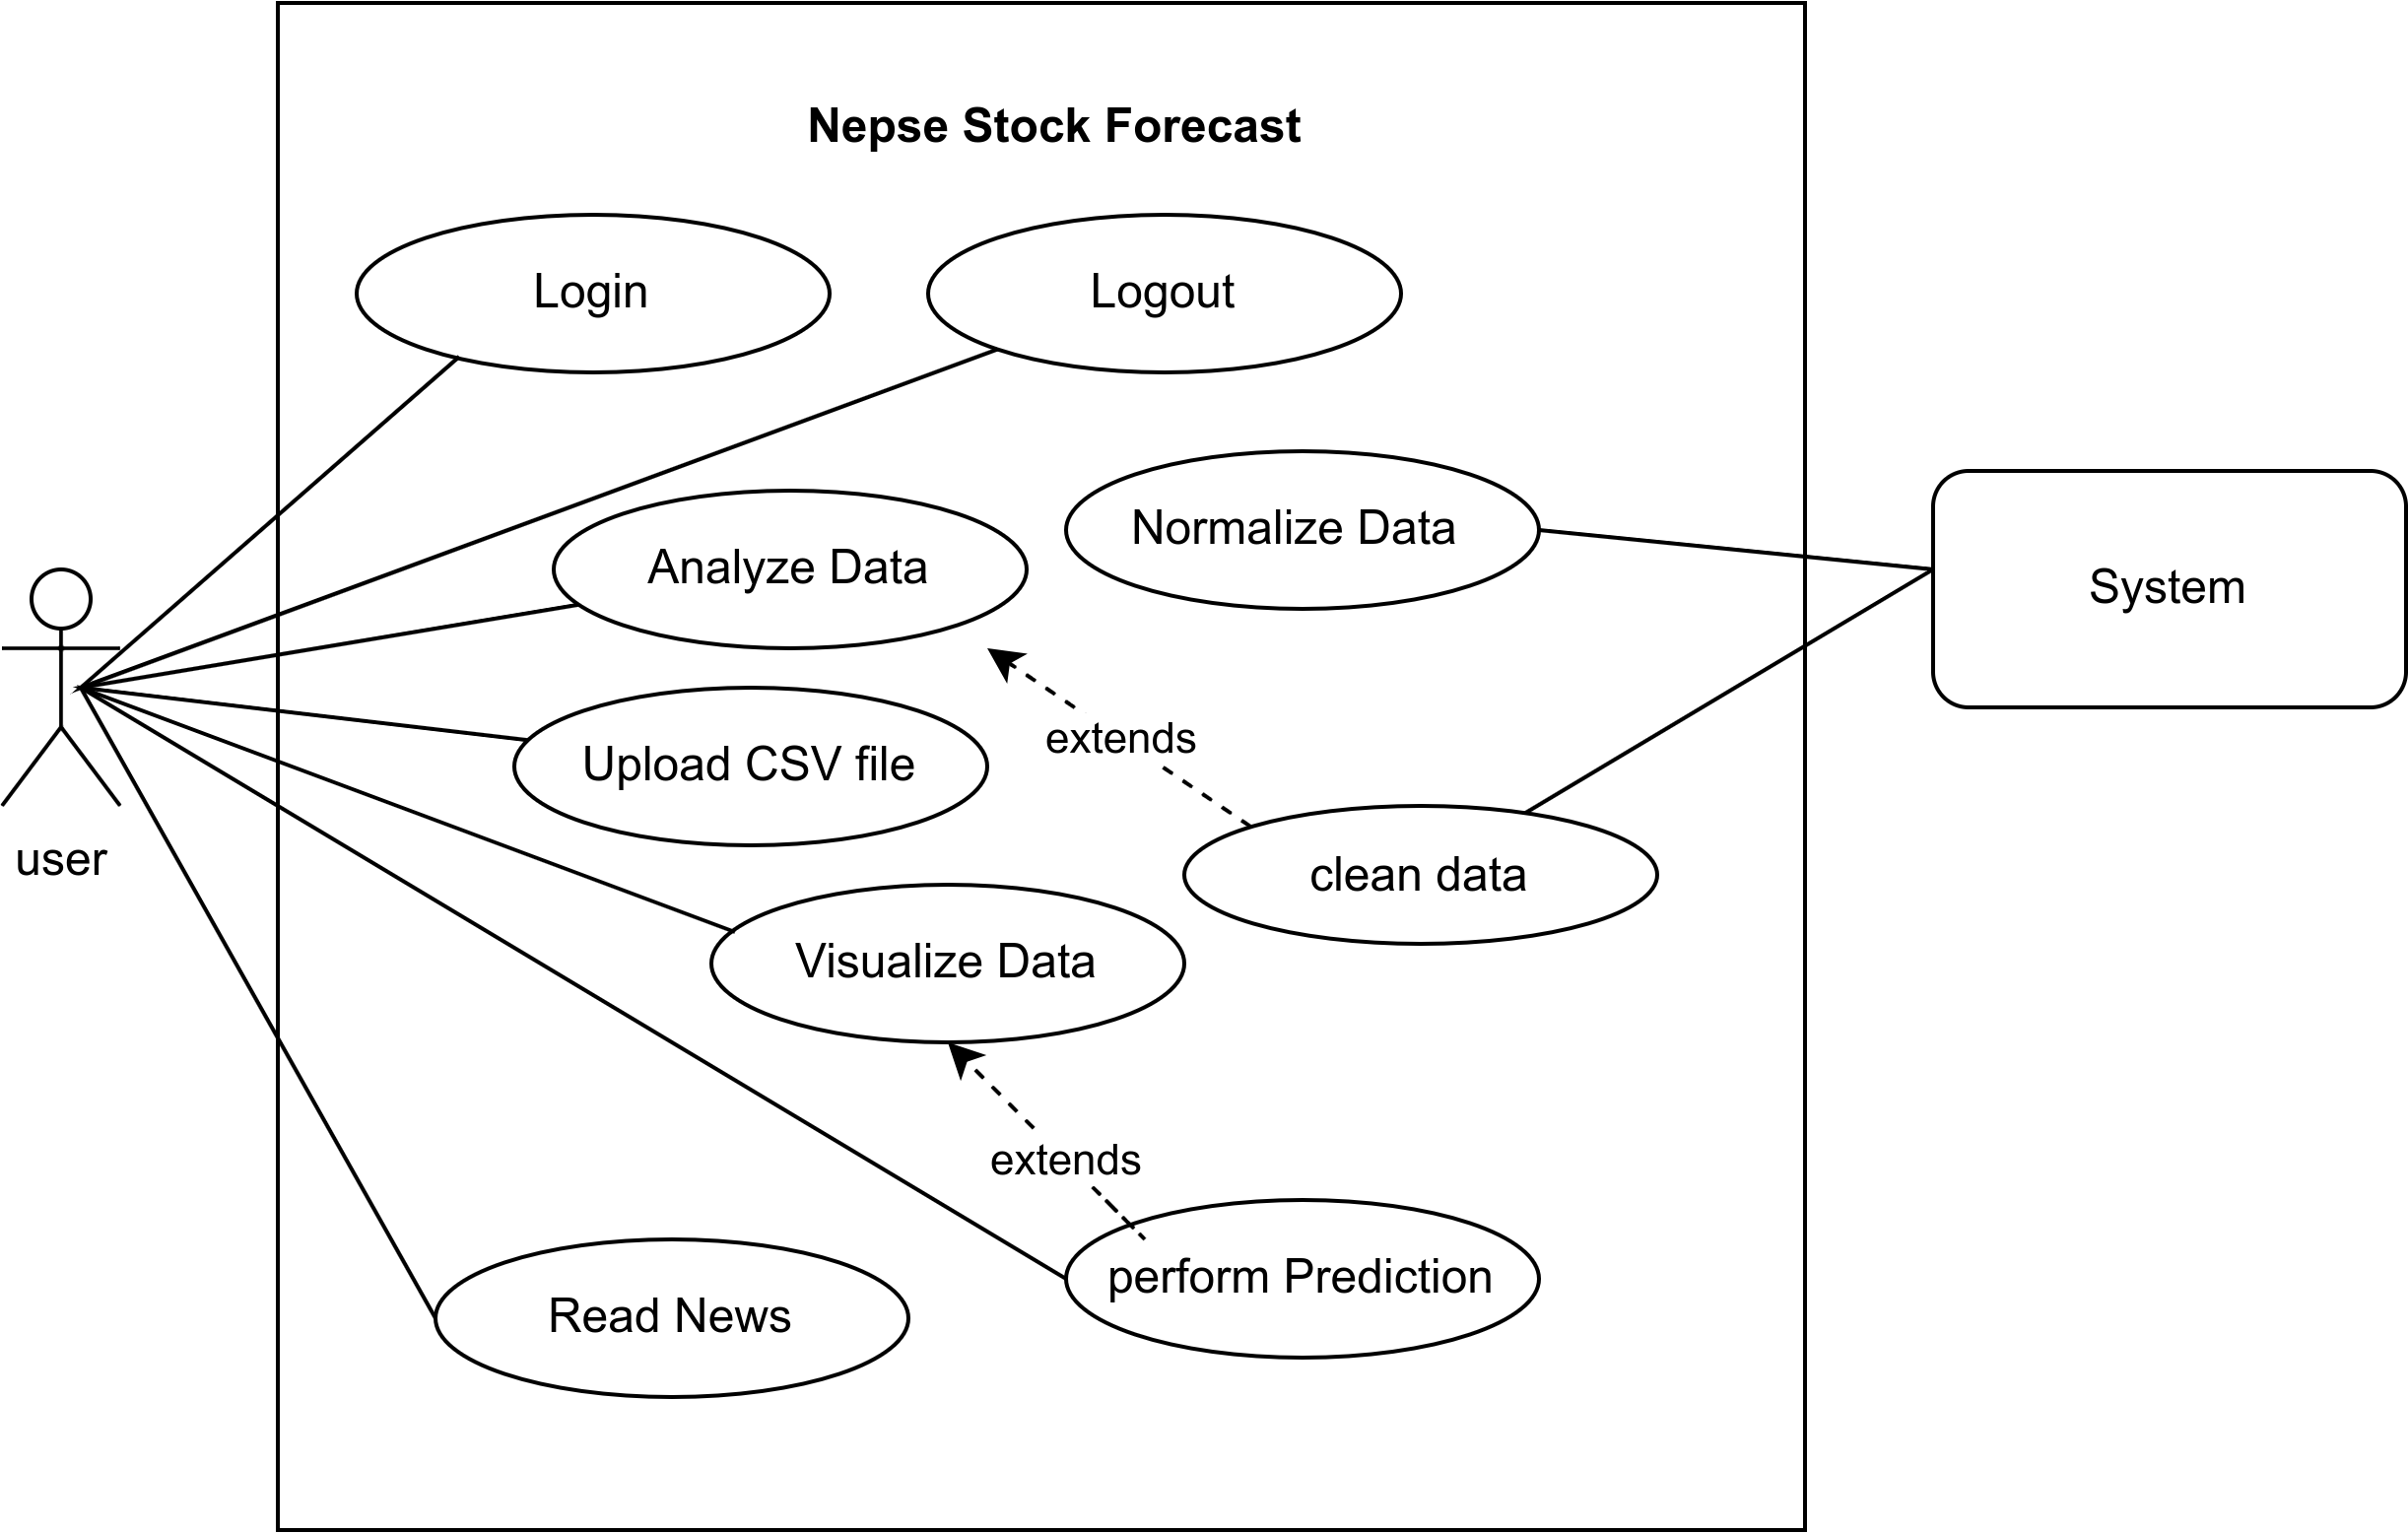
\includegraphics[width=1\linewidth]{images/Mideterm.png}
     \caption{Usecase Diagram}
     \label{fig:3.2}
 \end{figure}

 The Usecase Diagram shows the user interaction with the system and the system's response to the user's actions. The user can interact with the system by logging in, viewing stock data, and making predictions. The system will respond by providing the user with the requested data and predictions. The system will also provide visualizations of the historical and predicted stock prices.

\end{document}